\section{Deferred Explanations}
\label{sec:deferred-proofs}

\subsection{How a dealer is ``bound'' to a committed value}
\label{sec:dealer-bound-to-commited-value}

In section \ref{sec:building-blocks-for-the-protocol} we said that the dealer is bound to his shared value once he committed to it. Of course, there are several ways to implement this, but we will briefly describe one from \cite{lecture-notes-goldwasser-bellare}.

Therefore, we use some one-way collision-free hash function $H$ (a one-way function is a function that can be easily evaluated, but whose inverse is very complicated or impossible to compute). Then, if we want to commit to some value $x$, we can send as a ``promise'' the value $y=H(x)$. Note that -- informally spoken -- nobody is able (at least not in feasible time) to find another value $x\neq y$ with $H(x)=H(x')=y$.

This way, we are bound to the value $x$ since we published $y=H(x)$ already, but can not find another value that yields $y$ when we apply $H$ to it. Thus, if we later publish our secret $x$, the other players just need to check whether they obtain $y$ when they apply $H$ to it. This way, we can not change our mind without being caught.

\subsection{The basic idea of secret sharing}
\label{sec:appendix-basic-idea-secret-sharing}

Consider the following basic idea for secret sharing. Assume you have some bit $s$ that you want to share among three players such that no player con reconstruct the value on her own (but they should be able to reconstruct it altogether). 

Then, you could toss two coins yielding random bits $s_1$ and $s_2$. Moreover, you construct a third bit $s_3=s_1\oplus s_2\oplus s$. Note that then $s=s_1\oplus s_2 \oplus s_3$. Then you give $s_1$ to player 1, $s_2$ to player 2 and so forth. Afterwards the three players can -- collaboratively -- reconstruct the value $s$, but none of them can do so on her own.

This is -- of course -- a very simple scheme, that only works if all players are honest and if \emph{all} players join the collaborative computation.

However, there are more sophisticated techniques (e.g. relying on polynomials over finite fields like $\mathbb Z_p$ for some prime $p$) that allow a certain amount of dishonest players and still work. 

For more information on that topic, please refer to \cite{shamir_secret_sharing}.

\subsection{Collaborative coin flipping -- basic idea}
\label{sec:appendix-coin-flipping}

Taking the XOR (evaluating securely and secretly) of all these bits returns the random bit generated by all the participants in common. This computation (XOR on any number of bits) can be done in a constant number of rounds and using only polynomial amount of communication. This can be seen e.g. by a deeper investigation of the arguments in \cite{beaver-verifiable-secret-sharing} (according to \cite{Beaver1990}).

From now on, we use the symbol $\oplus$ to denote the XOR-computation. Even if XOR is usually defined on single bits only, we apply this function to bit strings bit-wise (e.g. $1100\oplus1001=0101$).

\subsection{Some words on Pseudorandom Generators}
\label{sec:appendix-pseudorandom-generators}

It is -- by today -- a widely known fact that pseudorandom generators exist if and only if so-called \emph{one-way} functions exist. These are functions that are easy to compute, but hard to invert. For more information on the relation between one-way functions and pseudorandom generators, please refer to \cite{lecture-notes-goldwasser-bellare,yao-theory-application-trapdoor-functions,pseudorandom-generators-blum}.

Up to now, it is an open question, whether such one-way functions exist. Thus, it is -- as mentioned in section \ref{sec:building-blocks-for-the-protocol} -- not proven that pseudorandom generators exist at all.

One remark that has to be made in this context is the following: The existence of one-way functions (or -- equivalently -- of pseudorandom generators) directly implies $\mathbf{P}\neq\mathbf{NP}$ ($\mathbf{P}$ and $\mathbf{NP}$ being the famous complexity classes, of course). This is simply, because the inverse of such a one-way function would be ``hard to compute, but easy to verify'', which is -- informally -- what $\mathbf{NP}$ is about.

Thus, a proof for the existence of pseudorandom generators is probably -- to put it mildly -- none of the simple-to-read ones.

\subsection{Size of two-fan-in-circuits}
\label{sec:size-two-fan-circuits}

We can reduce any circuit to a circuit consisting only of gates having two input wires, increasing its size only by a polynomial factor.

To prove this, consider an AND-gate having $n>2$ wires. Then, we can simulate this gate using only AND-gates with two input wires. 

We do this in a manner similar to a complete binary tree (see Figure \ref{fig:complete-binary-tree}). 

\begin{figure}[t]
  \centering
  \subfigure[A single AND-gate with eight inputs.]{
    \begin{tikzpicture}[xscale=3]
      \draw(0,0) rectangle (1.6,0.4);
      \draw[->, semithick] (0.1,-.4) -- (0.1,0);
      \draw[->, semithick] (0.3,-.4) -- (0.3,0);
      \draw[->, semithick] (0.5,-.4) -- (0.5,0);
      \draw[->, semithick] (0.7,-.4) -- (0.7,0);
      \draw[->, semithick] (0.9,-.4) -- (0.9,0);
      \draw[->, semithick] (1.1,-.4) -- (1.1,0);
      \draw[->, semithick] (1.3,-.4) -- (1.3,0);
      \draw[->, semithick] (1.5,-.4) -- (1.5,0);
      \draw[->, semithick] (.8,.4) -- (.8,1.4);
    \end{tikzpicture}
  }
  \hspace{1cm}
  \subfigure[Several 2-input AND gates simulate one 8-input AND gate.]{
  \centering
  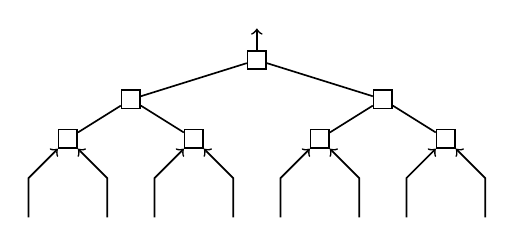
\begin{tikzpicture}
    [level distance=5mm, 
    level 1/.style={sibling distance=32mm},
    level 2/.style={sibling distance=16mm},
    level 3/.style={sibling distance=8mm},
    level 4/.style={sibling distance=4mm},
    semithick,
    every node/.style={draw=black,<-},
    %edge from parent fork down,
    ]
    \node[semithick] (root) {}
    child {node{} 
      child {node{}
      }
      child {node{}
      }
    }
    child {node{} 
      child {node{}
      }
      child {node{}}
    };
    % \draw[<-] (root-1-1-1) -- +(0,-.5);
    % \draw[<-] (root-1-1-2) -- +(0,-.5);
    % \draw[<-] (root-1-2-1) -- +(0,-.5);
    % \draw[<-] (root-1-2-2) -- +(0,-.5);
    % \draw[<-] (root-2-1-1) -- +(0,-.5);
    % \draw[<-] (root-2-1-2) -- +(0,-.5);
    \draw[<-] (root-1-1)   -- +(.5,-.5) -- +(.5,-1);
    \draw[<-] (root-1-1)   -- +(-.5,-.5) -- +(-.5,-1);
    \draw[<-] (root-1-2)   -- +(.5,-.5) -- +(.5,-1);
    \draw[<-] (root-1-2)   -- +(-.5,-.5) -- +(-.5,-1);
    \draw[<-] (root-2-1)   -- +(.5,-.5) -- +(.5,-1);
    \draw[<-] (root-2-1)   -- +(-.5,-.5) -- +(-.5,-1);
    \draw[<-] (root-2-2)   -- +(.5,-.5) -- +(.5,-1);
    \draw[<-] (root-2-2)   -- +(-.5,-.5) -- +(-.5,-1);
    \draw[->] (root) -- + (0,.4);
  \end{tikzpicture}
  }
  \caption{Simulating an $n$-input AND-gate by several 2-input AND-gates}
  \label{fig:complete-binary-tree}
\end{figure}

The bottom level consists of at most $\frac{n}{2}$ AND-gates. The second-to-bottom level consists of at most $\frac{n}{4}$ gates. The next level has at most $\frac{n}{8}$ gates, and so forth. Thus, the total number of gates used is at most $\sum_{i=1}^{\log n} \frac{n}{2^i}\leq n$.

Thus, for one AND-gate that has $n$ inputs, we can construct a sub-circuit consisting of at most $n$ gates such that this sub-circuit resembles the computation of the original AND-gate. The size increased by a polynomial factor (in the number of inputs of the original gate). 

For other types of gates, we can use similar constructions.

Since any gate can have at most as many inputs as there are gates in the whole circuit, the size of the total circuit increases by a polynomial factor in the size of the circuit.

Note that this idea does not only work for AND gates, but also for other gates. In particular, it is working for splitter gates (as introduced in section \ref{sec:introducing-splitters}).

\subsection{Why the use of Pseudorandom Generators?}
\label{sec:appendix-why-pseudorandom-generators}

Let us for a moment consider equation (\ref{eq:gate-label-definition-with-output}) and propose the following question: The output of $G_0$ resp. $G_1$ on some $k$-bit string is a binary string of length $nk+1$. So, one might argue that it would be simpler to work directly on the signals $\sigma=\sigma_1\dots\sigma_n a$ and $\tau=\tau_1\dots\tau_n b$ instead of first splitting up the signals into its components and then considering $G_b(\sigma_i)$ and $G_a(\tau_j)$, respectively.

While this simplification would be useful if we were just interested in correctness, but when this is done, we loose privacy. That is, a player possibly can deduce the semantics of some signals -- which is something we strictly wanted to prevent.

To see this, consider a simple AND-gate (input wires $\alpha$ and $\beta$, output wire $\gamma$). Assume we know the left incoming signal $\sigma^\alpha$ to represent semantics $\mathbf{0}$ and has parity $a$ (similar, $\sigma^\beta$ has parity $b$). Then, we can surely say that the outgoing signal $\sigma^\gamma$ is also $\mathbf{0}$. If we would directly operate on the signals (i.e. without random generators), we could -- since we know all table entries for the gate -- deduce the signal for $\beta$ with parity $1-b$ (by simply considering the table entry $A^g_{a(1-b)}$). That is, we then would know all signals for wire $\beta$.

Then we do the same the other way around and compute all signals for wire $\alpha$. This enables us to ``test'' the gate with all combinations of odd and even signals. Since we knew that $\sigma^\alpha$ had parity $a$ and semantics $\mathbf{0}$, we could without problems try the other signal for $\alpha$ and see if the value of the wire $\gamma$ changes. This would enable us to deduce the semantics for the input wire $\beta$.

On the other hand, if we use pseudorandom generators, we can not deduce all the other signals, since the values $A^g_{ab}$ are scrambled. This prevents us from simply reconstructing the signals (and, thus, the semantics).

\subsection{Why do we need splitters?}
\label{sec:appendix-splitters}

We illustrate the need for splitters by an example along \cite{Xu:2004:MAS:1023552}. Let us imagine the situation, where two parties hold two numbers $x_1$ and $x_2$ (each consisting of $l$ bits). The parties want to know the higher of the numbers, i.e. $\max(x_1,x_2)$.

Therefore, they could use a circuit as depicted in figure \ref{fig:max-of-numbers-xu-circuit}. It takes two $l$-bit inputs $x_1$ and $x_2$ and gives them to a comparator that outputs one bit \footnote{This output is shown as two separate wires, since it is used in several gates as input.}. This output is 1 if $x_1\geq x_2$, and 0 otherwise.

Moreover, it uses two \emph{masks}. A mask takes an $l$-bit input vector (in figure \ref{fig:max-of-numbers-xu-circuit}, depicted as the incoming wires from the bottom) and a single \emph{masking} bit (shown as a single wire from the side). Its output is a $l$-bit-vector. This vector holds zeroes only, if the masking bit is 0. Otherwise, the output vector is the same as the input vector.

\begin{figure}[t]
  \centering
  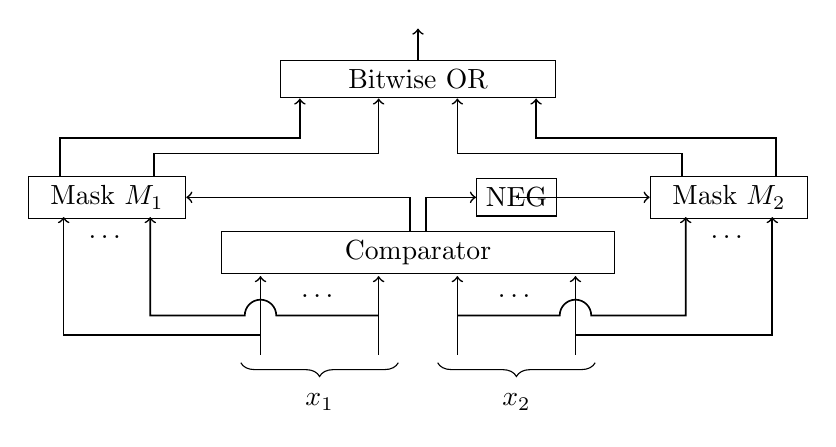
\begin{tikzpicture}
    \begin{scope}
      \draw[->,semithick] (-.25,-.50) -- (-.25,.5);
      \node at (.5,.25) {\dots};
      \draw[->,semithick] (1.25,-.50) -- (1.25,.5);
      \draw[decorate,decoration={brace,amplitude=0.5em}](1.5,-.6) -- (-.5,-.6);
      \node at (.5,-1.1) {$x_1$};
    \end{scope}
    \begin{scope}[xshift=2.5cm]
      \draw[->,semithick] (-.25,-.50) -- (-.25,.5); 
      \node at (.5,.25) {\dots}; 
      \draw[->,semithick] (1.25,-.50) -- (1.25,.5);
      \draw[decorate,decoration={brace,amplitude=0.5em}] (1.5,-.6) -- (-.5,-.6);
      \node at (.5,-1.1) {$x_2$};
    \end{scope}
    \node[shape=rectangle,minimum width=5cm,draw=black] (compi) at (1.75,.8) {Comparator};
    % x -> mask 1
    \draw[->,semithick] (-.25,-.25) -| +(-2.5,1.5);
    \node at (-2.2,1) {\dots};
    \draw[->,semithick] (1.25,0) -- ++(-1.3,0) arc(0:180:.2) -| +(-1.2,1.25);
    \node[shape=rectangle,draw=black,minimum width=2cm] (m1) at (-2.2,1.5) {Mask $M_1$};
    % y -> mask 2
    \begin{scope}[xshift=3.5cm,xscale=-1]
      \draw[->,semithick] (-.25,-.25) -| +(-2.5,1.5);
      \node at (-2.2,1) {\dots};
      \draw[->,semithick] (1.25,0) -- ++(-1.3,0) arc(0:180:.2) -| +(-1.2,1.25);+
      \node[shape=rectangle,draw=black] (neg) at (.5,1.5) {NEG};
      \node[shape=rectangle,draw=black,minimum width=2cm] (m2) at (-2.2,1.5) {Mask $M_2$};
    \end{scope}
    \draw[->,semithick] (compi.north)  +(-.1,0) |- (m1);
    \draw[->,semithick] (compi.north)  +( .1,0) |- (neg);    
    \draw[->,semithick] (neg) |- (m2);
    \node[shape=rectangle,draw=black,minimum width=3.5cm] (bo) at (1.75,3) {Bitwise OR};
    \coordinate[xshift=-.6cm] (m11) at (m1.north);
    \coordinate[xshift=.6cm] (m12) at (m1.north);
    \coordinate[xshift=-.6cm] (m21) at (m2.north);
    \coordinate[xshift=.6cm] (m22) at (m2.north);
    \draw[<-,semithick] (bo.south) +(-1.5,0) -- +(-1.5,-.5) -| (m11);
    \draw[<-,semithick] (bo.south) +(-0.5,0) -- +(-0.5,-.7) -| (m12);
    \draw[<-,semithick] (bo.south) +( .5,0) -- +( .5,-.7) -| (m21);
    \draw[<-,semithick] (bo.south) +(1.5,0) -- +(1.5,-.5) -| (m22);
    \draw[->,semithick] (bo.north) -- +(0,.4);
  \end{tikzpicture}
  \caption{A circuit representing the function $\max(x_1,x_2)$. This circuit has not the property that each wire is an used as an input wire at most once. Section \ref{sec:appendix-splitters} explains how this can be exploited by tackling the subcircuit $M_1$.}
  \label{fig:max-of-numbers-xu-circuit}
\end{figure}

Let us assume that the players already computed the outcome and saw that $x_2$ was the higher of the two numbers (i.e. player 2 had the higher number). We now consider what player 2 might do retrieve the value $x_1$ (which he was not supposed to learn).

Remember: We consider now what would happen if we would \emph{not} have used splitters, but instead just relied on the ``pure'' protocol described in \cite{Rogaway:1991:RCS:888502}.

The crucial part of this splitter-less garbled circuit is $M_1$, which is -- as a close-up -- depicted in figure \ref{fig:mask-m1}. This is a sub-circuit receiving input wires $\alpha_1,\dots,\alpha_l$ and one additional input wire $\beta$. Then each $\alpha_i$ is ANDed with $\beta$ and the results are ``returned'' as values $\gamma_i = \alpha_i \oplus \beta$. Note that in this case $\beta$ is participating in several different gates, since we did \emph{not} introduce splitters.

\begin{figure}[ht]
  \centering
  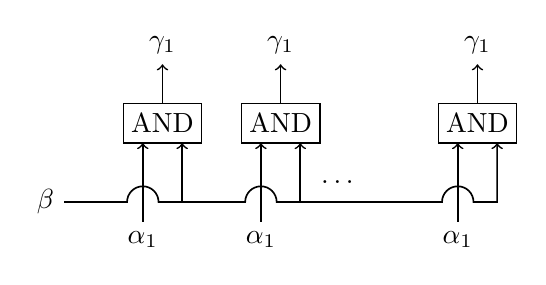
\begin{tikzpicture}
    \draw[->,semithick] (0,0) node[below]{$\alpha_{1}$} -- (0,1);
    \draw[->,semithick] (1.5,0) node[below]{$\alpha_{1}$} -- (1.5,1);
    \node at (2.5,.5) {\dots};
    \draw[->,semithick] (4,0) node[below]{$\alpha_{1}$} -- (4,1);
    \draw[->,semithick] (-1,.25) node[left] {$\beta$} -- (-.2,.25) arc(180:0:0.2) 
    -- (1.3,.25) arc(180:0:0.2) 
    -- (3.8,.25) arc(180:0:0.2) 
    -- (4.5,.25) -- (4.5,1);
    \draw[->,semithick] (.5,.25) -- (.5,1);
    \draw[->,semithick] (2,.25) -- (2,1);
    \draw(-.25,1)rectangle(.75,1.5);
    \draw(1.25,1)rectangle(2.25,1.5);
    \draw(3.75,1)rectangle(4.75,1.5);
    \draw[->,semithick](0.25,1.5) -- +(0,.5) node[above]{$\gamma_1$};
    \draw[->,semithick](1.75,1.5) -- +(0,.5) node[above]{$\gamma_1$};
    \draw[->,semithick](4.25,1.5) -- +(0,.5) node[above]{$\gamma_1$};
    \node at (0.25,1.25) {AND};
    \node at (1.75,1.25) {AND};
    \node at (4.25,1.25) {AND};
  \end{tikzpicture}
  \caption{The mask $M_1$ from the circuit in figure \ref{fig:max-of-numbers-xu-circuit}}. This sub-circuit can be exploited because one single wire -- namely wire $\beta$ -- participates in several gates.
  \label{fig:mask-m1}
\end{figure}

Player 2 already knows that his original number $x_2$ was at least as big as $x_1$. Now, he could try what would happen if $x_1$ would be zero\footnote{That is, essentially, player 2 asks himself: ``If $x_1'=0$, and I evaluate the circuit with $x_1'$ instead of $x_1$, what could I deduce?''}. We use a new variable $x_1'=0$ for that. In particular, player 2 sets (in his mind) every (plaintext) bit of $x_1'$ to 0. Note that he does not know the proper signals for these bits.

Since the circuit -- evaluated on $x_1$ and $x_2$ -- revealed some signals $\sigma^{\gamma_1},\dots,\sigma^{\gamma_l}$ to player 2, and we know that $x_2\geq x_1$, we know that the signals $\sigma^{\gamma_i}$ must represent semantics 0.

But if we supply $x_1'=00\dots 0$ instead of $x_1$ the signals $\sigma^{\gamma_i}$ must \emph{still} represent semantics 0 (since $M_1$ is essentially just a collection of AND-gates). This is true, even if we set $\beta$ to 1 -- we introduce again an additional variable $\beta'=1$ to denote which value we supply to the gates. That is, if we supply $\beta'$ and $x_1'$ to the sub-circuit, we still know the proper outgoing signals.

So, let us now consider the $i$-th AND-gate within $M_1$, and look what happens, if supply $\beta'$ and $x_1'$. Supplying $x_1'$ results in some signals $\varsigma^{\alpha_i}$. But we still know the proper output signal $\sigma^{\gamma_i}$.

We assume now that $b$ is the parity of the signal along wire $\beta$, and $a_i$ is the parity of signal on input wire $\alpha_i$. Then, for the AND-gate $g_i$, we can compute 
\begin{equation}
  \label{eq:mu_i-is-a-tricky-thing}
  \mu_i:=\sigma^{\gamma_i}\oplus G_b(s^{\alpha_i}_{a,1}) \oplus G_b(s^{\alpha_i}_{a,2}) \oplus A^{g_i}_{a_i b}.
\end{equation}

We consider the parts of the right-hand side:

\begin{itemize}
\item The values $\sigma^{\gamma_i}$ is known since it must represent semantics 0. Since we already evaluated the garbled circuit with $x_2\geq x_1$, we know these signals.
\item The outputs of our pseudorandom generator, $G_b(s^{\alpha_i}_{a,1})$ and $G_b(s^{\alpha_i}_{a,2})$, are known because we know the signals along wires $\alpha_i$ and can just compute the output of the pseudorandom generators $G_0$ and $G_1$ on the respective inputs.
\item The gate labels $A^{g_i}_{a_i b}$ are trivially known since they are part of the garbled circuit.
\end{itemize}

As you can see, we can compute the vales $\mu_i$ without any further complications.

Now comes a key insight: If our guess for the $i$-th bit of $x_1$ was correct (i.e. if $\sigma^{\alpha_i} = \varsigma^{\alpha_i}$), then $\sigma^{\gamma_i}$ is the correct outgoing signal (for the $i$-th bit of $x_1'$). Remember that we constructed the gate labels as in equation (\ref{eqn:gate-labels-definition}). Using this definition, we can deduce that $\mu_i=G_a(s^\beta_{b1})\oplus G_a(s^\beta_{b2})$. That is, then the value $\mu_i$ depends essentially only on the signal along the wire $\beta$ (we can evaluate $G_0$ and $G_1$ without problems).

If our guess was incorrect, $\mu_i$ will be some random binary string.

This means: If we guessed the $i$-th bit of $x_1$ correct, then $\mu_i$ will be either $G_0(s^\beta_{b1})\oplus G_0(s^\beta_{b2})$ or $G_1(s^\beta_{b1})\oplus G_1(s^\beta_{b2})$. 

Now, we can do the following: Note that -- in a collection of random, sufficiently long bit-strings -- the probability that a string occurs twice is rather low. But in our collection of values $\mu_i$, there might well be duplicate vales -- the ones for whom our guess of the $i$-th bit was correct. So, we collect all the values $\mu_i$ and sort them into certain ``groups'' the following way: We collect values that occur multiple times and group them. The remaining strings form the last group.

That is, in the first and second group, all the values $\mu_i$ are collected that are probably generated by $G_0(s^\beta_{b1})\oplus G_0(s^\beta_{b2})$ or $G_1(s^\beta_{b1})\oplus G_1(s^\beta_{b2})$, respectively. The third group contains all the other, random strings. All indices in the third group correspond to the bits that were wrongly guessed. Thus, these bits are probably 1 (since we guessed 0). The indices in the other groups are the correctly-guessed ones.

It can be shown that the probability that we obtain the correct bits of $x_1$ using this technique, is rather high -- too high to be acceptable in a cryptographic setting.

The weakness exploited here lay in the fact that one single value -- the signal along wire $\beta$ (resp. the output of a pseudorandom generator applied to it) -- took part in several other gates.

If we now use splitters, this ensures that not one single signal participates in several gates, but this single signal is duplicated into many other \emph{random} signals, so one can not exploit the shown inter-gate dependencies.

Of course, this is just a very superficial treatment of this topic. For an in-depth proof, of all the statements, we refer to \cite{Xu:2004:MAS:1023552}.

%%% Local Variables: 
%%% mode: latex
%%% TeX-master: "seminar"
%%% End: 